\documentclass[11pt,a4paper]{article}
\usepackage[latin5]{inputenc}
\usepackage[english]{babel}
\usepackage{amsmath}
\usepackage{amsfonts}
\usepackage{amssymb}
\usepackage{graphicx,subfig}
\usepackage{placeins}
\usepackage{gensymb}

\author{Alexander Attinger, Yannic Kilcher}
\title{Report Sheet 2, Advanced Part}

\begin{document}
\maketitle


\section{Generalized Hough Transform}
\paragraph{Gabor Filters}
The generalized Hough transform is an algorithm used to detect custom shapes. We implemented our own version of the algorithm, roughly following the steps	from the provided resources. To obtain a look up table, following steps were performed with an image of the template shape:
\begin{enumerate}
\item generate an 'edge mask' using Canny Edge filter
\item filter image with gaussian filter
\item calculate gradient direction for each edge pixel using sobel operators
\item for each edge pixel, calculate the difference vector to a reference pixel (set by user)
\item generate the look up table containing for each direction bin all the corresponding difference vectors
\end{enumerate}

We used an arbitrary shape (see Fig. \ref{fig:1}) and the letter F as template (see Fig. \ref{fig:2}). To detect a shape in an image following steps were performed on the test image:

\begin{enumerate}
\item calculate gradient direction for each pixel
\item for the obtained angle, retrieve all the difference vectors from the look up table
\item add each vector seperately to the current pixel, increasing the score in a seperate image by one at the resulting location, see Figures \ref{fig:3} and \ref{fig:4} for the resulting maps
\item perform a thresholding operation on the maps to get the points with the highest scores. These points correspond to detected objects.
\end{enumerate}

\begin{figure}
\centering
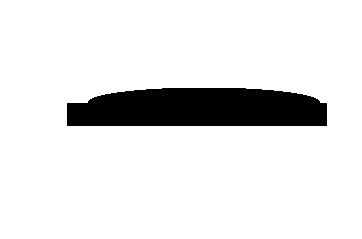
\includegraphics[scale=.4]{img/templateShape.png}

\caption{Arbitrary shape used as template}
\label{fig:1}
\end{figure}

\begin{figure}
\centering

\includegraphics[scale=.4]{img/templateLetter.png}

\caption{Letter shape used as template}
\label{fig:2}
\end{figure}

\begin{figure}
\centering
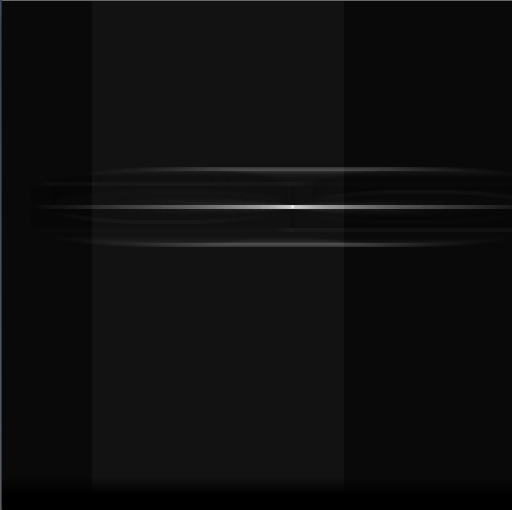
\includegraphics[scale=.4]{img/mapTemplate.png}

\caption{Response map of the hough transform using the shape from \ref{fig:1} as template and the same image as test image.}
\label{fig:3}
\end{figure}

\begin{figure}
\centering
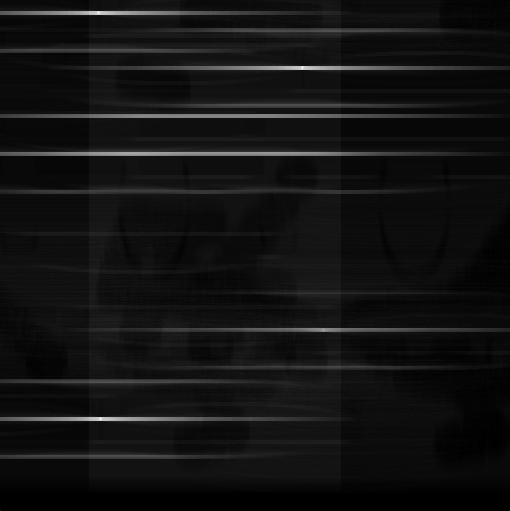
\includegraphics[scale=.4]{img/mapShape.png}

\caption{Response map of the hough transform using the shape from \ref{fig:1} as template. The image shown in figure \ref{fig:6} was used as test image}
\label{fig:4}
\end{figure}


\begin{figure}
\centering
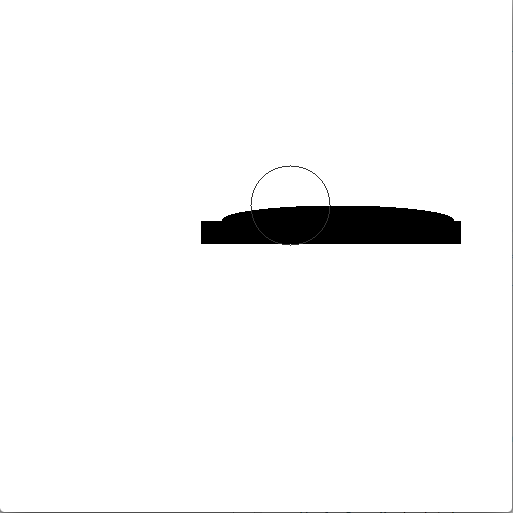
\includegraphics[scale=.4]{img/matchTemplate.png}

\caption{The hough transform detects the own template image well. The circle is drawn around the detected reference point (which is the same as the original reference point. The reference point is not in the center of the object, therefor the circle is also not at the center.  }
\label{fig:5}
\end{figure}

\begin{figure}
\centering
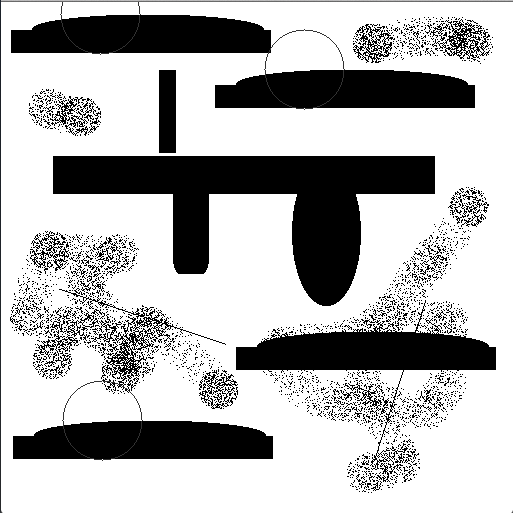
\includegraphics[scale=.4]{img/matchShape.png}

\caption{Detected instances of the shape in a more complex scene. It was detected three times (marked by circle), one of the instances, occluded by speckles and a line was not detected.  }
\label{fig:6}
\end{figure}

\begin{figure}
\centering
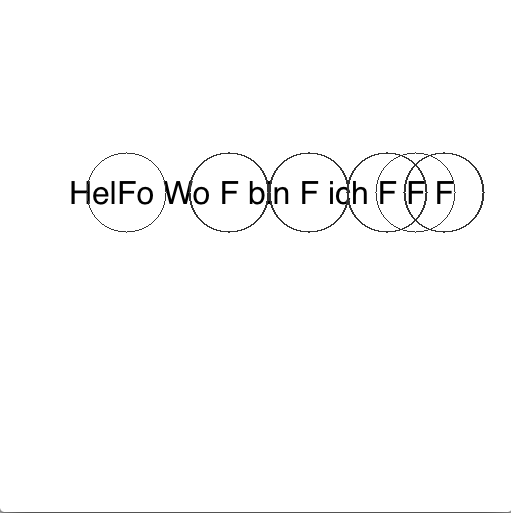
\includegraphics[scale=.4]{img/matchLetter.png}

\caption{Detected letters F (marked with a circle) in a sentence. }
\label{fig:7}
\end{figure}

\paragraph{Discussion}










\end{document}
